\documentclass[letterpaper]{article}

% --- Required Packages ---
\usepackage{parskip}            % Removes paragraph indentation, adds space between paragraphs
\usepackage[unicode, draft=false]{hyperref} % Setup hyperref package, and colours for links
\usepackage{titlesec}           % For custom section formatting
\usepackage{fancyhdr}           % Required for custom headers and footers
\usepackage{extramarks}         % Required for \lastxmark in the footer
\usepackage{enumitem}           % For nice lists (bullet points)
\usepackage[backend=biber, style=numeric]{biblatex}
\usepackage{amsmath}            % Required for algorithm block
\usepackage{algorithm}          % Required for algorithm wrapper
\usepackage[noend]{algpseudocode} % Required for algorithm block
\usepackage{tikz} 
\usepackage{array}
\usepackage{tabularx}
\usepackage[table]{xcolor}
\usetikzlibrary{calc, positioning, arrows.meta}
\addbibresource{references.bib}
\RequirePackage{graphicx}

% --- Lab Details Variables ---
\newcommand{\labTitle}{Lab \#3: Security and Privacy Issues in ML}
\newcommand{\labDueDate}{April 20th, 2026}
\newcommand{\labClass}{CSC429}
\newcommand{\labClassTime}{}
\newcommand{\labClassInstructor}{Professor Fang}
\newcommand{\labAuthorName}{\textbf{Helen Huy, McCay Rudick, Jess Alencaster}}

% --- Basic Document Settings ---
\topmargin=-0.45in
\evensidemargin=0in
\oddsidemargin=0in
\textwidth=6.5in
\textheight=9.0in
\headsep=0.25in

\linespread{1.1}

% --- Header and Footer Settings ---
\pagestyle{fancy}
\lhead{\labAuthorName}
\rhead{\labClass\ : \labTitle}
\lfoot{\lastxmark}
\cfoot{\thepage}

\renewcommand\headrulewidth{0.4pt}
\renewcommand\footrulewidth{0.4pt}

\setlength\parindent{0pt}

% --- Custom Section Formatting  ---
\titleformat{\section}{\Large\bfseries\raggedright}{}{0em}{}[\titlerule]
\titlespacing{\section}{0pt}{10pt}{5pt}
\titleformat{\subsection}{\large\bfseries\raggedright}{}{0em}{}
\titlespacing{\subsection}{0pt}{8pt}{3pt}

\begin{document}
\thispagestyle{empty}

% --- Title Block ---

\vspace*{\fill}
\begin{center}
    {\Huge \scshape \labTitle} \\ \vspace{10pt}
    {\Large \labAuthorName} \\ \vspace{5pt}
    {\large \labClassInstructor \ \labClassTime} \\ \vspace{5pt}
    {\large Due Date: \labDueDate}
\end{center} 
\vspace*{\fill}

\newpage
% BEGIN LAB CONTENT

\section{1. Security and Privacy Issues in ML-Based Systems}

\subsection*{Privacy Issue: Membership Inference Attacks (MIA)}
\textbf{Link:} \href{https://ieeexplore.ieee.org/abstract/document/8835245}{Comprehensive Privacy Analysis of Deep Learning \cite{nasr2019}} \\
\textbf{Description:} Machine learning models inadvertently memorize training data through the Stochastic Gradient Descent (SGD) algorithm. Thus, an adversary can analyze gradients to determine if a specific person's data was used to train the model \cite{nasr2019}. This works remarkably well even on well-generalized models; for example, DenseNet leaked 74.3\% accuracy under white-box conditions.

\textbf{Active inference attacks (subvariant of MIA):} In federated learning (FL), a malicious participant or parameter server can deliberately manipulate gradient updates (e.g., via gradient ascent). This forces the model to expose other participants' private data, achieving up to 92.1\% attack accuracy on AlexNet and 87.3\% on DenseNet \cite{nasr2019}, well above the 50\% random-guess baseline.

\begin{table}[h!]
\centering
\begin{tabular}{|l|l|l|l|}
\hline
\textbf{Privacy Issue} & \textbf{Attack Type} & \textbf{AlexNet} & \textbf{DenseNet} \\ \hline
1) MIAs (Passive) & White-box (gradients) & 75.1\% & 74.3\% \\ \hline
2) Active Inference Attacks (in FL) & Malicious aggregator (ascent + isolation) & 92.1\% & 87.3\% \\ \hline
\end{tabular}
\caption{MIA Attack Accuracies \cite{nasr2019}}
\end{table}

\textbf{How are MIA attacks launched?} \\
ML models trained with SGD leave a footprint in their parameters for every training point, turning the model itself into a privacy leak. Even after training concludes, an adversary can run a target data point through the model and compute the gradient $g=\nabla_{W}L$. They then feed $g$, the model output $f(x)$, and label $y$ into a pre-trained attack model $h$. If $||g||\approx0$, the point was likely a training member \cite{nasr2019}.

\begin{algorithm}[h!]
\caption{White-box Membership Inference Attack \cite{nasr2019}}
\begin{algorithmic}[1]
\State \textbf{Input:} model $f$, point $x$, label $y$
\State \textbf{Output:} $\hat{m} \in \{0,1\}$ \quad {\small($1 =$ member, $0 =$ non-member)}
\State $g \leftarrow \nabla_{W}\,\mathcal{L}(f(x;W), y)$ \quad {\small (backpropagate)}
\State \Return $h(g,\, f(x),\, y)$ \quad {\small($||g|| \approx 0 \Rightarrow$ member)}
\end{algorithmic}
\end{algorithm}


\pagebreak

\subsection*{Security Issue: Data Poisoning Attacks}
\textbf{Link:} \href{https://www.ndss-symposium.org/wp-content/uploads/2020/04/diss2020-23003-paper.pdf}{Poisoning Attacks on FL-based IoT IDS \cite{nguyen2020}} \\
\textbf{Description:} Data poisoning attacks corrupt an ML model by injecting malicious data into the training process. In an FL-based Intrusion Detection System (IDS), this manifests as a backdoor attack: attackers gradually inject malicious traffic into training data via compromised IoT devices, blinding the detector so it misclassifies malicious traffic as benign \cite{nguyen2020}.

\textbf{How are data poisoning attacks launched?} \\
Data poisoning is a strategic execution rather than a single algorithm:
\begin{enumerate}
    \item The attacker compromises IoT devices across multiple local networks (no gateway compromise needed).
    \item They inject malicious traffic into the benign training stream at a controlled Poisoned Data Rate (PDR).
    \item The Security Gateway unknowingly trains on poisoned data, backdooring its local model.
    \item Poisoned local models are sent to the aggregator and averaged into the global model.
    \item The corrupted global model now misclassifies malicious traffic as benign across all gateways.
\end{enumerate}

\begin{figure}[h!]
\centering
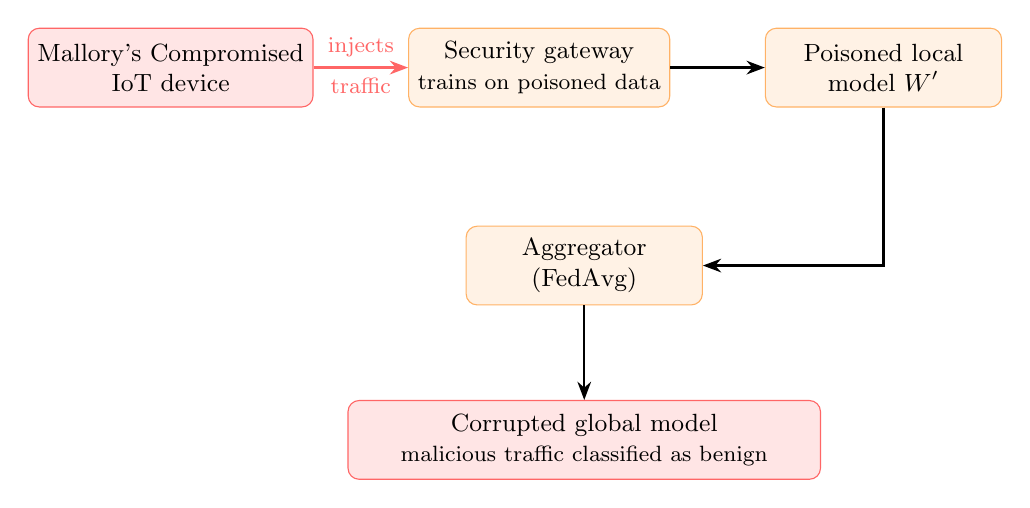
\begin{tikzpicture}[
  node distance=1.5cm,
  box/.style={rectangle, rounded corners=4pt, minimum width=3cm, minimum height=1cm, text centered, draw, font=\small, align=center},
  redbox/.style={box, fill=red!10, draw=red!60},
  amberbox/.style={box, fill=orange!10, draw=orange!60},
  arr/.style={->, >=Stealth, thick}
]
\node[redbox] (iot) {Mallory's Compromised\\IoT device};
\node[amberbox, right=1.2cm of iot] (gw) {Security gateway\\{\footnotesize trains on poisoned data}};
\node[amberbox, right=1.2cm of gw] (local) {Poisoned local\\model $W'$};
\node[amberbox, below=1.5cm of local, xshift=-3.8cm] (agg) {Aggregator\\(FedAvg)};
\node[redbox, below=1.2cm of agg, minimum width=6cm] (global) {Corrupted global model\\{\footnotesize malicious traffic classified as benign}};

\draw[arr, red!60] (iot) -- node[above]{\footnotesize injects} node[below]{\footnotesize traffic} (gw);
\draw[arr] (gw) -- (local);
\draw[arr] (local) |- (agg);
\draw[arr] (agg) -- (global);
\end{tikzpicture}
\caption{Backdoor Data Poisoning Attack Flow, adapted from Nguyen et al. (2020) \cite{nguyen2020}}
\end{figure}

\textbf{Why are data poisoning attacks dangerous?} \\
By design, they are stealthy. Even after the global model is backdoored, it continues to classify normal traffic correctly, giving operators no indication of compromise. Even when differential privacy defenses are applied, the attack still achieves 100\% backdoor accuracy, while only dropping normal traffic detection to 94.2\% \cite{nguyen2020}. Furthermore, this specific poisoning attack, unlike conventional poisoning attacks, only requires control of IoT devices, which are inherently vulnerable due to their limited computing capability, minimal built-in security, and low-cost hardware, where 50\% of commercially available IoT devices contain significant security flaws \cite{sadhu2022}. Thus, in the context of IoT devices, this attack is far more practical to execute in real-world deployments compared to conventional poisoning approaches.
\pagebreak

\section{2. Solutions and Applicable Platforms}

\subsection*{Solutions to Identified Vulnerabilities}
\begin{itemize}
    \item \textbf{Solution for MIA (Differential Privacy):} To mitigate Membership Inference Attacks (MIA), Differential Privacy (DP) can be integrated into the Stochastic Gradient Descent (SGD) algorithm \cite{abadi2016}. By mathematically clipping the per-sample gradient to bound its sensitivity, then injecting calibrated Gaussian noise into the updates, the system obscures the footprint of any single data point. This makes it mathematically improbable for an attacker to conclude if $||g|| \approx 0$, meaning an attacker cannot be certain that a specific user's information was part of the training set.
    \item \textbf{Solution for Data Poisoning (Federated Learning + Advanced Aggregation):} Raw data exposure is greatly reduced with the introduction of Federated Learning (FL). However, the aggregation phase is still vulnerable to poisoned local models. To solve this, an advanced aggregation method must be used (such as Trimmed Mean \cite{yin2018}) rather than standard FedAvg. This approach helps detect and filter statistical outliers (the poisoned gradients) before they can be merged into the global IDS.
\end{itemize}

\subsection*{Applicable Platform}
\textbf{Platform:} \textbf{TensorFlow Privacy} (\href{https://www.tensorflow.org/responsible_ai/privacy/guide}{TensorFlow Privacy Guide}). \\
TensorFlow Privacy is an open-source library built on TensorFlow. It can implement DP-SGD, the exact mechanism described in our MIA solution above. It provides built-in gradient clipping, Gaussian noise injection, and the ``moments accountant'' that tracks the cumulative privacy budget ($\epsilon$, $\delta$) across training steps \cite{abadi2016}. 

Using this platform, we can demonstrate MIA vulnerability through the following steps:
\begin{enumerate}
    \item Train a Convolutional Neural Network (CNN) without DP to expose gradient leakage.
    \item Apply DP-SGD with varying $\epsilon$ values to represent different privacy budgets.
    \item Observe how increasing noise reduces MIA attack accuracy at the cost of model utility.
\end{enumerate}
All of these steps allow us to practically study the privacy-utility tradeoff.
\pagebreak

\section{3. Modeling the System: Membership Inference Attacks}

\subsection*{System Model}
We extend the Federated Learning-based IoT IDS proposed by Nguyen et al. (2020) \cite{nguyen2020} by replacing their GRU-based local model with a 1D-CNN architecture as implemented by Torre et al. (2025) \cite{torre2025}. In this architecture, distributed Security Gateways collaborate with a central Aggregator to train a global anomaly detection model without ever exposing the raw IoT traffic data.

Specifically, the block diagram of this architecture and its attack surface is illustrated in Figure 2:

\begin{figure}[h!]
\centering
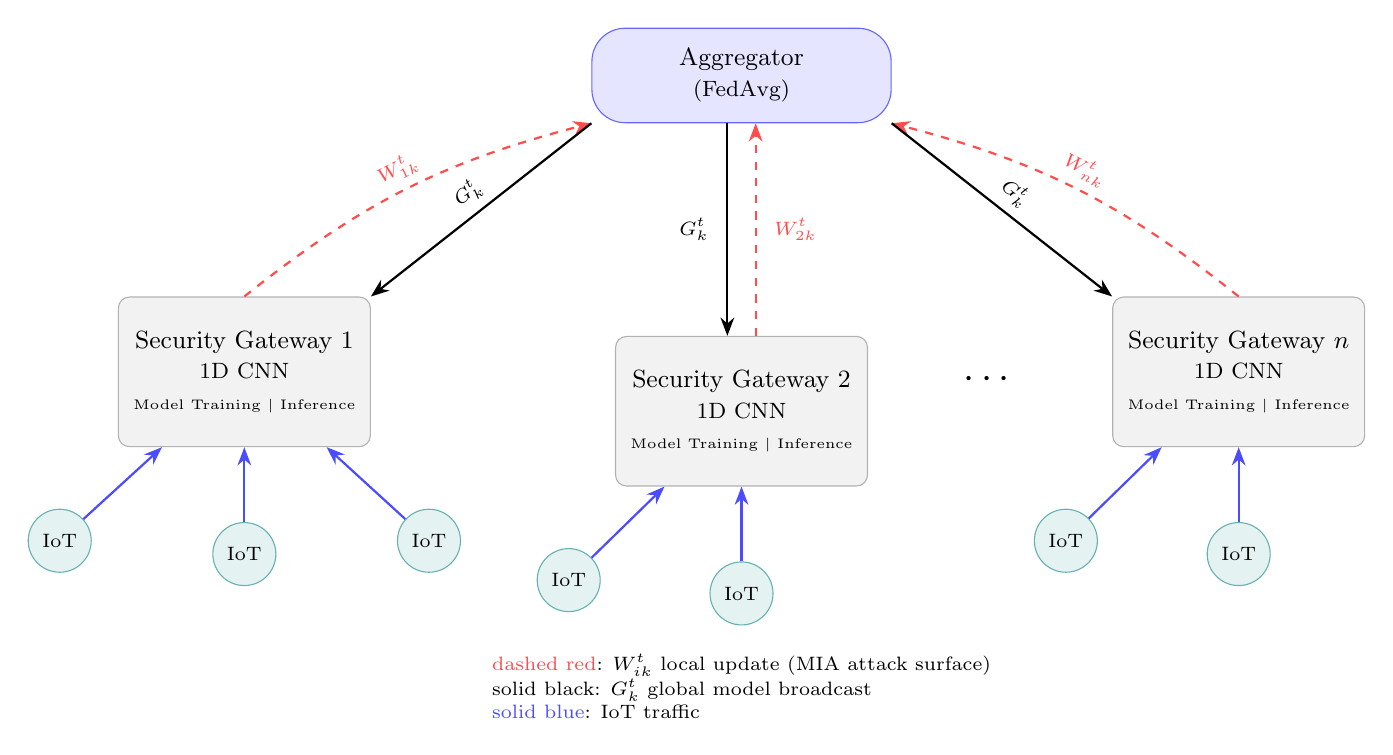
\begin{tikzpicture}[
    node distance=1.5cm,
    aggregator/.style={
        rectangle,
        rounded corners=12pt,
        draw=blue!60,
        fill=blue!10,
        minimum width=3.8cm,
        minimum height=1.2cm,
        font=\small,
        align=center
    },
    gateway/.style={
        rectangle,
        rounded corners=4pt,
        draw=gray!60,
        fill=gray!10,
        minimum width=3.2cm,
        minimum height=1.9cm,
        font=\small,
        align=center
    },
    iot/.style={
        circle,
        draw=teal!60,
        fill=teal!10,
        minimum size=8mm,
        font=\scriptsize
    },
    globalarr/.style={->, >=Stealth, thick},
    localarr/.style={->, >=Stealth, thick, red!70, dashed},
    trafficarr/.style={->, >=Stealth, thick, blue!70}
]

% Aggregator
\node[aggregator] (agg) {Aggregator\\{\footnotesize (FedAvg)}};

% Gateways
\node[gateway, below left=2.2cm and 2.8cm of agg] (gw1)
{Security Gateway 1\\{\footnotesize 1D CNN}\\{\tiny Model Training $\mid$ Inference}};

\node[gateway, below=2.7cm of agg] (gw2)
{Security Gateway 2\\{\footnotesize 1D CNN}\\{\tiny Model Training $\mid$ Inference}};

\node[gateway, below right=2.2cm and 2.8cm of agg] (gw3)
{Security Gateway $n$\\{\footnotesize 1D CNN}\\{\tiny Model Training $\mid$ Inference}};

% Ellipsis
\node[font=\Large] at ($(gw2)!0.5!(gw3)+(0,0.15)$) {$\cdots$};

% IoT devices
\node[iot, below left=0.9cm and 0.45cm of gw1] (iot1a) {IoT};
\node[iot, below=0.95cm of gw1] (iot1b) {IoT};
\node[iot, below right=0.9cm and 0.45cm of gw1] (iot1c) {IoT};

\node[iot, below left=0.9cm and 0.3cm of gw2] (iot2a) {IoT};
\node[iot, below=0.95cm of gw2] (iot2b) {IoT};

\node[iot, below left=0.9cm and 0.3cm of gw3] (iot3a) {IoT};
\node[iot, below=0.95cm of gw3] (iot3b) {IoT};

% IoT traffic to gateways
\draw[trafficarr] (iot1a) -- (gw1);
\draw[trafficarr] (iot1b) -- (gw1);
\draw[trafficarr] (iot1c) -- (gw1);

\draw[trafficarr] (iot2a) -- (gw2);
\draw[trafficarr] (iot2b) -- (gw2);

\draw[trafficarr] (iot3a) -- (gw3);
\draw[trafficarr] (iot3b) -- (gw3);

% Local updates to aggregator (MIA surface)
\draw[localarr]
    (gw1.north) to[bend left=12]
    node[midway, above, sloped, font=\scriptsize, text=red!70] {$W_{1k}^t$}
    (agg.south west);

\draw[localarr]
    ($(gw2.north)+(0.18,0)$) --
    node[midway, right, xshift=3pt, font=\scriptsize, text=red!70] {$W_{2k}^t$}
    ($(agg.south)+(0.18,0)$);

\draw[localarr]
    (gw3.north) to[bend right=12]
    node[midway, above, sloped, font=\scriptsize, text=red!70] {$W_{nk}^t$}
    (agg.south east);

% Global model broadcasts BCK to gateways
\draw[globalarr]
    (agg.south west) --
    node[midway, above, sloped, font=\scriptsize] {$G_k^t$}
    (gw1.north east);

\draw[globalarr]
    ($(agg.south)+(-0.18,0)$) --
    node[midway, left, xshift=-3pt, font=\scriptsize] {$G_k^t$}
    ($(gw2.north)+(-0.18,0)$);

\draw[globalarr]
    (agg.south east) --
    node[midway, above, sloped, font=\scriptsize] {$G_k^t$}
    (gw3.north west);

% Legend below figure
\node[align=left, font=\scriptsize, anchor=north] at ($(gw2.south)+(0,-2.0cm)$) {
\textcolor{red!70}{dashed red}: $W_{ik}^t$ local update (MIA attack surface)\\
\textcolor{black}{solid black}: $G_k^t$ global model broadcast\\
\textcolor{blue!70}{solid blue}: IoT traffic
};
\end{tikzpicture}

\caption{System Model for FL-based IoT IDS under MIA, combining architectures from Nguyen et al. (2020) \cite{nguyen2020} and Torre et al. (2025) \cite{torre2025}.}
\end{figure}

\pagebreak

\subsection*{Trust Model}
We then consider the honest-but-curious aggregator threat scenario. We adopt the standard FL assumption that the aggregator correctly follows aggregation protocols to maintain the global model, but may passively exploit the local model updates it receives to infer private membership information about individual training data points \cite{nasr2019}. The trust relationships between system components are summarized below in Table \ref{tab:trust-model}.

\vspace{1em}
\renewcommand{\arraystretch}{1.5}
\begin{table}[h!]
\centering
\begin{tabularx}{\textwidth}{|
    >{\raggedright\arraybackslash}p{0.27\textwidth}|
    >{\raggedright\arraybackslash}p{0.20\textwidth}|
    >{\raggedright\arraybackslash}p{0.18\textwidth}|
    >{\raggedright\arraybackslash}X|}
\hline
\rowcolor{black}
\centering\arraybackslash\textcolor{white}{\textbf{Entity}} &
\centering\arraybackslash\textcolor{white}{\textbf{Trusted By}} &
\centering\arraybackslash\textcolor{white}{\textbf{Trust Level}} &
\centering\arraybackslash\textcolor{white}{\textbf{Rationale}} \\
\hline

IoT devices &
Security Gateway &
Full &
IoT devices connect to their local gateway by design with no adversarial competition. \\
\hline

Security Gateway &
Aggregator &
Partial &
Gateways must submit updates but cannot verify the aggregator is not curious. \\
\hline

Aggregator &
$W_{ik}^{t}$ (local updates) &
Untrusted &
Curious aggregator exploits gradient updates to infer private membership \cite{nasr2019}. \\
\hline

Security Gateway &
$G_{k}^{t}$ (global model) &
Full &
Gateways accept \textbf{AND} deploy the global model to perform local inference. \\
\hline

Security Gateway &
Security Gateway &
None &
Participants cannot observe each other’s updates. Only the aggregated global model is visible. \\
\hline
\end{tabularx}
\caption{Trust relationships in federated intrusion detection setting.}
\label{tab:trust-model}
\end{table}

\pagebreak

\subsection*{Threat Model}
\begin{itemize}
    \item \textbf{Adversary Goal:} The adversary aims to determine whether a specific IoT traffic record, say $x$, was included in some private training dataset $D_{ik}$ of a target Security Gateway $i$. Formally, the adversary seeks to compute the membership prediction $\hat{m} \in \{0,1\}$, where $\hat{m}=1$ indicates that $x \in D_{ik}$ and $\hat{m}=0$ indicates otherwise. In this IoT IDS context, this allows the adversary to infer sensitive behavioral information about users whose devices generated the traffic.

    \item \textbf{Adversary Capability:} This adversary is an honest-but-curious aggregator that correctly executes FedAvg, but passively observes all local model updates $W_{ik}^t$ uploaded by Security Gateways across some $T$ training rounds. The adversary does not disrupt the protocol, compromise any Security Gateway, or inject malicious updates.

    \item \textbf{Adversary Knowledge:} The adversary operates within a white-box setting. Therefore, it has full access to the 1D CNN architecture, model parameters, and the per-layer gradient vectors $g=\nabla_{W}\mathcal{L}(f(x;W),y)$, computed from the uploaded local updates. Importantly, this gradient access is the key enabler of MIA, as later CNN layers retain some distinguishable gradient ``footprints'' for training membership versus non-members \cite{nasr2019}.

    \item \textbf{Attack Vector:} The attack vector is the gradient upload channel. Specifically, this consists of the local model updates $W_{ik}^t$ uploaded by each Security Gateway to the Aggregator during the training phase. As we illustrate in Figure 1, SGD forces $||g||$ toward zero for training members. This creates a statistically distinguishable signal that the adversary can exploit via some pre-trained attack model, say $h(g, f(x), y)$.

    \item \textbf{Assumptions:} We assume all Security Gateways are honest. Further, we assume the adversary controls no Security Gateways and does not modify the aggregation protocol. The adversary's advantage here comes solely from passive observation of gradient uploads over multiple training rounds.
\end{itemize}

% --- References ---
\newpage
\section{}

\printbibliography[title={References}]

\end{document}